\section{重要学术软件安装}
\subsection{安装及配置matlab}
(1) 配置Matlab使用的Java环境
\begin{verbatim}
$ sudo update-alternatives --config java
$ export MATLAB_JAVA=/usr/lib/jvm/java-6-sun-1.6.0.20/jre/
\end{verbatim}

(2) 挂载iso文件 

\verb"$ sudo mount -o loop Mathworks.Matlab.R2012a.UNIX.iso /mnt"

(3) 跳转到挂载目录

\verb"$ cd /mnt"

(4) 安装 

\verb"$ sudo ./install"

(5) 安装中选择“不使用Internet安装”

(6) 窗口界面默认安装位置为 /usr/local/MATLAB/R2012a

(7) 接受许可协议

(8) 输入安装密钥:

\verb"37176-43568-09521-61284-60764-48411-11831-17282-31342-18748-48552-26727-08411"

(9) 安装类型选择“自定义”

(10) 点击“安装”进行安装

(11) 倒入许可协议($/mnt/crack/lic\_standalone.dat$)

(12) 等待安装结束

(13) 设置快捷方式

1.将附件里的matlab.desktop文件放在 /usr/share/applications 下,图片matlab.png放在/usr/share/icons

2.建立软链接 sudo ln -s /usr/local/MATLAB/R2012a/bin/matlab /usr/bin/matlab

(14) 解决中文乱码问题

1. 字体显示美化 

进入Matlab,从菜单打开:Files->preferences,打开Fonts页,把右边最下面的复选框Use antialising to smooth desktop fonts选中,重启MATLAB,字体显示的效果就很好了.

2.MATLAB使用自带的Java运行环境,根据CPU架构的不同,相对应的字体配置文件路径为:

32位版本 /usr/local/matlab/sys/java/jre/glnx86/jre/lib/fontconfig.properties

64位版本 /usr/local/matlab/sys/java/jre/glnxa64/jre/lib/fontconfig.properties

下面以32位版本为例

3.进入字体配置文件目录 cd /usr/local/MATLAB/R2012a/sys/java/jre/glnx86/jre/lib

如果fontconfig.properties文件不存在,可以从fontconfig.properties.src复制一个

sudo cp fontconfig.properties.src fontconfig.properties

4.字体可直接用系统自带的文泉驿

修改JRE的字体配置文件,打开配置文件: sudo gedit fontconfig.propertie

加入中文字体定义,在version=1下面一行输入

allfonts.chinese-arphic1=-misc-simsun-medium-r-normal--0-0-0-0-p-0-iso10646-1

如果文件已有allfonts.chinese-arphic1这行,就直接把它们改成上面那样。

指明中文字体路径,在allfonts.chinese-arphic1行后回车另起一行,输入中文字体文件的完整路径:filename.-misc-simsun-medium-r-normal--0-0-0-0-p-0-iso10646-1=/usr/share/fonts/truetype/wqy/wqy-microhei.ttc

5.修改字体搜索, 在配置文件中查找sequence.allfonts,如果其后的sequence开头的行中有: chinese-arphics1,可以略过此步,否则在其后面加入一行:sequence.fallback=chinese-arphic1

(15) 解决/usr/bin/matlab: 1: /usr/local/MATLAB/R2012a/bin/util/oscheck.sh: /lib/libc.so.6: not found

对于32位系统:

\verb" sudo ln -s /lib/i386-linux-gnu/libc.so.6 /lib/libc.so.6"

对于64位系统:

\verb" sudo ln -s /lib/x86_64-linux-gnu/libc.so.6 /lib64/libc.so.6"

\subsection{Vmware安装及配置}

\subsection{Virtualbox安装及配置}
(1) 双击deb文件进行安装

(2) 选择对应版本的extension包进行安装

(3) I'm on Ubuntu 12.04 64-bit and encountered exactly this problem. What finally worked was going to the virtualbox website, downloading the package and installing it via:

sudo apt-get purge virtualbox dkms linux-headers-\$(uname -r)

sudo apt-get install linux-headers-\$(uname -r)

sudo dpkg -i virtualbox-4.2\_4.2.10-84104~Ubuntu~precise\_amd64.deb

Then I ran:

sudo /etc/init.d/vboxdrv setup

And it worked like a charm.


\subsection{Cuda模拟器Ocelot的安装及配置}
(1) 建议使用svn checkout 最新的trunk
\verb"$ sudo svn checkout http://gpuocelot.googlecode.com/svn/trunk/ gpuocelot"
 
(2) 安装各种依赖包和库
\begin{verbatim}
sudo apt-get install flex bison autoconf automake libtool  g++
sudo apt-get install libboost1.40-all-dev
sudo apt-get install  libglu1-mesa-dev freeglut3-dev mesa-common-dev 
\end{verbatim}

上面一行是安装图形库GL,这个在后面cuda sdk 编译的时候会用到,反正安着也没坏处。我开始在安装ocelot的同时,手贱也去玩barra,安barra得注意几个包,因为需要直接和cuda sdk肉搏,常被告知 /usr/bin/ld 找不到 lxxx, 直接sudo apt-get install libxxx-dev就是了。

(3) 这些其实就可以进行正常编译了,当然,如果还想安装hydrazine也是可以的。
\begin{verbatim}
$ svn checkout http://hydrazine.googlecode.com/svn/trunk/ hydrazine
$ cd hydrazine
$ libtoolize; aclocal; autoconf; automake
$ ./configure;make;make check
$ sudo make install
\end{verbatim}

(4) 编译ocelot
\begin{verbatim}
$ cd gpuocelot/ocelot
$ libtoolize; aclocal; autoconf; automake
$ ./configure;make
\end{verbatim}

建议进行安装,要不在后续进行regression test 时,它会要你回来安装的

\verb"$ sudo make install"

但是这里注意,还需要安装cuda toolkit,最好版本匹配,就是说,你要进行cuda2.2的sdk 做测试,就最好安装2.2版本的tookit。

(5) 安装cuda 2.2 tookit

\verb"$ gedit ~/.bashrc"

添加:
\begin{verbatim}
PATH=/usr/local/cuda/bin:$PATH
LD_LIBRARY_PATH=/usr/local/cuda/lib:$LD_LIBRARY_PATH
\end{verbatim}

(6) 进行regression test
\begin{verbatim}
$ cd ../gpuocelot/tests/cuda2.2
$ libtoolize;aclocal; autoconf; automake
$ ./configure; make; make check
\end{verbatim}

在make check 这一步常会出错,错误大致为:“/usr/include/c++/4.4/new:91: error: 'operator new' takes type 'size\_t' ('unsigned int') as first parameter,”这个错误我在测试cuda2.3 和 cuda3.2的时候都出现过,很是无语,gcc.gnu.org说这是一个bug,我不知道如何应对,但是对于cuda2.2没有出现这个错误。

(7) 测试安装

\verb"$  make test"

\subsection{Cadence,Allegro和MMSIM的安装}

\subsection{Mathematica的安装}

\subsection{MPICh2的安装}
(1) 下载MPICH2并使用下面命令解压
\begin{verbatim}
      tar xzf mpich2-1.3.2.tar.gz
      cd mpich2-1.3.2
\end{verbatim}

(2) 选择安装目录/home/<USERNAME>/mpich2-install, <USERNAME>改为您的用户名,并确保安装目录为空或不存在。

(3) 将 MPICH2配置到指定的安装目录:
\begin{verbatim}
  $ sudo mkdir /usr/local/mpich2
    $ ./configure --prefix=/usr/local/mpich2 2>&1 | tee c.txt
\end{verbatim}

(4) 编译MPICH2:

\verb"$ make 2>&1 | tee m.txt"

(5) 安装 MPICH2 命令:

\verb"$ make install 2>&1 | tee mi.txt"

(6) 将安装目录中bin子目录添加到你的启动脚本中(.bashrc for bash):

\verb"PATH=/usr/local/mpich2/bin:$PATH ; export PATH"

用以下命令进行命令的检查:
\begin{verbatim}
        which mpicc
        which mpiexec
\end{verbatim}

这些命令应该显示出你安装目录的bin子路经.

(7) 使用下面命令测试安装是否成功<number>为要是用的cpu数目:

\verb"$ mpiexec -n <number> ./examples/cpi"

\subsection{Modelsim的安装}
(1) 直接运行

\verb"$ ./install.linux"

如果权限不够,添加权限  

\verb"$ sudo chmod a+x install.linux"

由于是图形界面,很easy。

如果出现下面的错误:
\begin{verbatim}
  Exception in thread "main" java.lang.UnsatisfiedLinkError:
   /home/happy/mgc/install.ixl/JRE/lib/i386/xawt/libmawt.so: libXtst.so.6: 
   cannot open shared object file: No such file or directory
\end{verbatim}

说明是在64位系统上运行了32位的Java,因此还需要安装以下软件包:

\verb"$ sudo apt-get install libxtst6:i386 libxi6 libxrender1"

(2) 破解

修改license.src和mentor文件,将前两行的SERVER和VENDER的信息按照Linux系统进行修改。
\begin{verbatim}
  SERVER HostName MACADDR 27001
  VENDOR mgcld /path-to-modelsim/modeltech/linux/mgcld
\end{verbatim}

  安装wine aptitude install wine

  运行wine MentorKG.exe 生成LIENCE.TXT

  添加license到path里面
\begin{verbatim}
  vim ~/.bashrc
  export LM_LICENSE_FILE=[license存放目录]/LICENSE.TXT   
  export PATH=$PATH:[modelsim安装目录]/bin
  source ~/.bashrc
\end{verbatim}

  在ubuntu 12.04上需要修改modeltech/bin/vsim文件的204行,增加

\verb\ 3.[1-9].[0-9]*)    vco="linux" ;;\

将crack/linux中的三个文件拷贝到Modelsim的安装目录Modelsim/modeltech/linux/mgls/lib目录中,然后运行$patch\_2013$中的命令:

\verb"./sfk6 rep -yes -pat -bin /5589E557565381ECD00000008B5508/31C0C357565381ECD00000008B5508/ -dir ./"

如果在输出的信息中出现
\begin{verbatim}
  [total hits/matching patterns/non-matching patterns]
  error: failed to read+write: sfk6 - skipping
  [001/1/0] mgcld                                                               
  [001/1/0] mgls_asynch                                                         
  5 files checked, 2 changed.
  1 errors occurred.
\end{verbatim}

  说明破解是成功的。如果是0 files checked,  在ubuntu下加sudo试试。

  (3) 运行

\verb"$ vsim"

  如果不能创建文件,考虑权限问题.如果在64位系统中出现下面的错误

\verb"  error while loading shared libraries: libXft.so.2"

  则运行下面的命令

\verb"$ sudo apt-get install ia32-libs"

\subsection{Nero的安装}

(1) 双击deb文件进行安装

\subsection{NS2的安装}
(1) 首先需要安装的是:
\begin{verbatim}
  sudo apt-get install build-essential
  sudo apt-get install tcl8.4 tcl8.4-dev tk8.4 tk8.4-dev
  sduo apt-get install libxmu-dev libxmu-headers
\end{verbatim}

  (2) 把解压缩后的资料夹移动到你想安装的位置去
\begin{verbatim}
  $ tar xvfz ns-allinone-2.31.tar.gz
  $ sudo mv ns-allinone-2.31 /usr/local/NS2
  $ sudo chmod 777 -R NS2
  $ cd /usr/local/NS2
  $ ./install
\end{verbatim}

  经过一些时间的等待,就会看到他显示一串要你修改.bashrc或.cshrc的讯息,依照提示信息加入。如果是.bashrc的话就会是:
\begin{verbatim}
  export PATH=$PATH:/usr/local/NS2/bin:/usr/local/NS2/tcl8.5.10/unix:/usr/local/NS2/tk8.5.10/unix
  export LD_LIBRARY_PATH=$LD_LIBRARY_PATH:/usr/local/NS2/otcl-1.14:/usr/local/NS2/lib
  export TCL_LIBRARY=$TCL_LIBRARY:/usr/local/NS2/tcl8.5.10/library
\end{verbatim}

(3) 接着依照最后几行的讯息,去做验证,例如:

\verb"$ cd ns-2.31; ./validate"

  当ns回车出现%说明正确。

\subsection{OMNet++的安装}
(1) 安装必要的软件:
\begin{verbatim}
  $ sudo apt-get install build-essential gcc g++ bison flex perl \      
  tcl-dev tk-dev blt libxml2-dev zlib1g-dev openjdk-6-jre \      
  doxygen graphviz openmpi-bin libopenmpi-dev libpcap-dev
\end{verbatim}

(2) 添加环境变量:

在.bashrc中增加如下代码:
\begin{verbatim}
  export PATH=/home/happy/omnet++-4.4.1/bin:$PATH
  export TCL_LIBRARY=/usr/share/tcltk/tcl8.5
\end{verbatim}

  (3) 配置、编译和安装:
\begin{verbatim}
  $ ./configure
  $ make
\end{verbatim}

\subsection{SystemC-2.2的安装(SystemC-2.3可以直接安装)}
1. Either install a Linux system natively or install a Virtual machine (VirtualBox) (recommended).

2. Download systemc-2.2.0.tgz 

3. tar -xvf systemc-2.2.0.tgz

4. cd systemc-2.2.0

5. configure --prefix=/usr/local/systemc-2.2

6. sudo mkdir /usr/local/systemc-2.2

7.0. add '\#include <cstdlib>' and '\#include <string.h>' before '\#include "sysc/utils/sc\_report.h"' in systemc-2.2.0/src/sysc/utils/sc\_utils\_ids.cpp

7.1 error: reference 'm\_obj' cannot be declared 'mutable' [-fpermissive]

这个错误信息有好几行连续的,找到sc\_bit\_proxies.h,将那几行中的mutable都删去即可。

8. make (ignore the complilation error of example code)

9. sudo make install

10. add newline with expression:
\begin{verbatim}
  SYSTEMC_HOME=”/usr/local/systemc-2.2/“ in /etc/environment
  export SYSTEMC_HOME=/usr/local/systemc-2.2/
\end{verbatim}

11. To compile a systemC program simply use this expression: 

g++ -I. -I$SYSTEMC\_HOME/include -L. -L$SYSTEMC\_HOME/lib-linux -o sim hello.cpp -lsystemc -lm %32 bit OS

g++ -I. -I$SYSTEMC\_HOME/include -L. -L$SYSTEMC\_HOME/lib-linux64 -o sim hello.cpp -lsystemc -lm %64 bit OS
  
the example code:
\begin{verbatim}
  // All systemc modules should include systemc.h header file
  #include "systemc.h"
  // Hello_world is module name
  SC_MODULE (hello_world) {
    SC_CTOR (hello_world) {
      // Nothing in constructor 
    }
    void say_hello() {
      //Print "Hello World" to the console.
      cout << "Hello World.\n";
    }
  };
  // sc_main in top level function like in C++ main
  int sc_main(int argc, char* argv[]) {
    hello_world hello("HELLO");
    // Print the hello world
    hello.say_hello();
    return(0);
  }
\end{verbatim}

\subsection{SoCLib的安装}

\subsection{TeX Live 2011 安装步骤}
CTEX 有 TexLive (TexLive为Latex安装包的名字)的所有内容,还包括了中文的支持。但是在Linux环境下没有对应的ctex安装包.

第一步:准备

我是使用光盘镜像安装TeX Live 2011,所以在安装前需要准备如下材料:

TeX Live 2011光盘镜像,Windows字体(从Windows 系统拷贝),Adobe字体(网络下载)

第二步:开始安装(采用GUI安装方式)

首先安装 perl-tk

\verb"$ sudo aptitude install perl-tk"

挂载 TeX Live 2011 镜像
\begin{verbatim}
    sudo mkdir /mnt/iso
    sudo mount -o loop texlive2011.iso /mnt/iso
\end{verbatim}

安装

\verb"$ sudo /mnt/iso/install-tl --gui"

第三步:安装TeX Live 2011

信息读取完毕后,探出一个界面如下:
\begin{figure}
\centering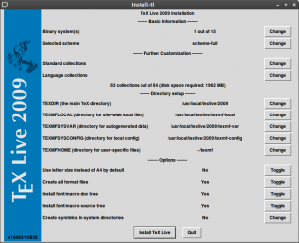
\includegraphics[scale=0.7]{figures/texlive.png}
\caption{Texlive安装界面}\label{texlive}
\end{figure}
    
我把最后一项“自动创建链接”修改外,其他保持原样。点击“安装TeX Live“。

第四步:配置环境变量

我的默认shell 是bash.一次对照安装指南。打开终端,输入:

vi ~/.profile或者vim /etc/bash.bashrc

然后把以下代码添加进去(注意path一定要将texlive放在前面)
\begin{verbatim}
       PATH=/usr/local/texlive/2011/bin/i386‐linux:$PATH; export PATH
       MANPATH=/usr/local/texlive/2011/texmf/doc/man:$MANPATH; export MANPATH
         INFOPATH=/usr/local/texlive/2011/texmf/doc/info:$INFOPATH; export INFOPATH
\end{verbatim}

接着,修改/etc/manpath.config    

\verb"$ sudo  vi /etc/manpath.config"

在\# set up PATH to MANPATH mapping下输入
\verb" MANPATH_MAP /usr/local/texlive/2011/bin/i386-linux /usr/local/texlive/2011/texmf/doc/man"

第五步:配置中文环境和中文字体安装

首先:创建Windows字体目录WinFonts和Adobe字体目录AdobeFonts
\begin{verbatim}
    sudo mkdir /usr/share/fonts/WinFonts
    sudo mkdir /usr/share/fonts/AdobeFonts
\end{verbatim}

第二 复制上述准备的字体到各自目录.这里需要注意:修改上面拷贝字体的权限 
\begin{verbatim}
              sudo chmod 644 /usr/share/fonts/WinFonts/*
              sudo chmod 644 /usr/share/fonts/AdobeFonts/*
\end{verbatim}

如果没有这一步,会在编译tex文件时出现下面类似的错误:
\verb" SimSun at 17.28pt not loadable"

第三 刷新字体缓存
\begin{verbatim}
    sudo  mkfontscale
    sudo mkfontdir
    sudo fc-cache -fsv
\end{verbatim}

第六步:安装中文字体后的配置

首先,查看系统中安装的中文字体的名字。

\verb"$ fc-list :lang=zh | sort"

第二, 查看并根据生成的 fonts 编辑 ctex-xecjk-winfonts.def

\verb"$ sudo  vi/usr/local/texlive/2011/texmf-dist/tex/latex/ctex/fontset/ctex-xecjk-winfonts.def"

编辑前ctex-xecjk-winfonts.def如下:
\begin{verbatim}
  % ctex-xecjk-winfonts.def: Windows 的 xeCJK 字体设置,默认为六种中文字体
  %vim:ft=tex
  \setCJKmainfont[BoldFont={SimHei},ItalicFont={[simkai.ttf]}]  
    {SimSun}
    \setCJKsansfont{SimHei}
    \setCJKmonofont{[simfang.ttf]}
    \setCJKfamilyfont{zhsong}{SimSun}
    \setCJKfamilyfont{zhhei}{SimHei}
    \setCJKfamilyfont{zhkai}{[simkai.ttf]}
    \setCJKfamilyfont{zhfs}{[simfang.ttf]}
    \newcommand*{\songti}{\CJKfamily{zhsong}} % 宋体
    \newcommand*{\heiti}{\CJKfamily{zhhei}}   % 黑体
    \newcommand*{\kaishu}{\CJKfamily{zhkai}}  % 楷书
    \newcommand*{\fangsong}{\CJKfamily{zhfs}} % 仿宋
    \newcommand*{\lishu}{\CJKfamily{zhli}}    % 隶书
    \newcommand*{\youyuan}{\CJKfamily{zhyou}} % 幼圆
    \endinput
\end{verbatim}

其中带中括号的字体名都是需要修改的,这时需运行

\verb"$ fc-list :lang=zh-cn"

来查看系统中的中文字体,记下楷体和仿宋对应的名称,即显示信息中第一个英文在我的系统中楷体是 KaiTi,仿宋是 FangSong不过会因为安装的字体版本不同而有所差异.

接下来只要将对应的字体修改即可,即把[SIMKAI.TTF]修改为KaiTi,把[SIMFANG.TTF]修改为FangSong,编辑后 ctex-xecjk-winfonts.def 的内容:
\begin{verbatim}
      % ctex-xecjk-winfonts.def: Windows 的 xeCJK 字体,默认六种中易字体
 	% vim:ft=tex
    \setCJKmainfont[BoldFont={SimHei},ItalicFont={KaiTi}]  {SimSun}
    \setCJKsansfont{SimHei}
    \setCJKmonofont{FangSong}
    \setCJKfamilyfont{zhsong}{SimSun}
    \setCJKfamilyfont{zhhei}{SimHei}
    \setCJKfamilyfont{zhkai}{KaiTi}
    \setCJKfamilyfont{zhfs}{FangSong}
    \setCJKfamilyfont{zhli}{LiSu}
    \setCJKfamilyfont{zhyou}{YouYuan}
    \newcommand*{\songti}{\CJKfamily{zhsong}} % 宋体
    \newcommand*{\heiti}{\CJKfamily{zhhei}}   % 黑体
    \newcommand*{\kaishu}{\CJKfamily{zhkai}}  % 楷书
    \newcommand*{\fangsong}{\CJKfamily{zhfs}} % 仿宋
    \newcommand*{\lishu}{\CJKfamily{zhli}}    % 隶书
    \newcommand*{\youyuan}{\CJKfamily{zhyou}} % 幼圆
    \endinput
\end{verbatim}

第三 ctex-xecjk-adobefonts.def不用改。

第四.sudo   tlmgr   install   xeCJK   ctex

第八步:测试

输入一个典型的中文支持例子测试,用xelatex或pdflatex命令编译
\begin{verbatim}
    \documentclass[UTF8]{ctexart}    
	\begin{document}    
	这是我的第一个\TeX{}文件    
	\end{document}
\end{verbatim}

第九步:安装texmaker

\verb"$ sudo apt-get install texmaker"

\subsection{安装Cuda}

\subsection{安装Android开发环境}

\subsection{安装Blender软件}

\subsection{安装Bochs软件}

\subsection{安装Docear}

\subsection{安装glimpse}

\subsection{安装gephi}

\subsection{安装IDA Pro}

\subsection{安装Jabref}

\subsection{安装Ruby}
\verb"$ sudo apt-get install ruby irb rdoc"

\subsection{安装lxr}

\subsection{安装Maple}

\subsection{安装Tomcat}
(1)	下载连接http://java.sun.com/javase/downloads/index.jsp

选择jdk-6u3-linux-i586.bin下载(可以下载最新的,但要注意一定不能是....i586-rpm.bin,一般Ubuntu下没有rpm工具),将jdk-6u3-linux-i586.bin放置于任意目录下如:/home/test

(2)更改文件权限为可执行、解压:
\begin{verbatim}
  cd /home/test
  chmod u+x jdk-6u3-linux-i586.bin
  sudo ./jdk-6u3-linux-i586.bin yes/no选择yes,执行完之后边可
\end{verbatim}

以在test目录下面看到文件夹jdk1.6.0\_03

(3) 设置环境变量
\begin{verbatim}
  sudo vi /etc/profile   在profile文件最后添加
  JAVA_HOME=/home/test/jdk1.6.0_03
  export JRE_HOME=$JAVA_HOME/jre
  export CLASSPATH=$JAVA_HOME/lib:$JRE_HOME/lib:$CLASSPATH
  export PATH=$JAVA_HOME/bin:$JRE_HOME/bin:$PATH
\end{verbatim}

保存并关闭

(4) 重启系统 (也可以不用重启系统先logout然后login)

(5) 查看java版本

在终端输入java -version将会显示java版本的相关信息,jdk安装成功

(6) 下载tomcat 6 http://apache.etoak.com/tomcat/tomcat-6/v6.0.20/bin/apache-tomcat-6.0.20.tar.gz

(7) 解压:tar zxvf apache-tomcat-6.0.20.tar.gz 就会在同一目录下产生 apache-tomcat-6.0.20文件夹;可以把apache-tomcat-6.0.20 拷贝到任意目录;

\begin{verbatim}
    sudo cp -r apache-tomcat-6.0.20 /var/tomcat6
  cd /var/tomcat6/bin
  sudo ./startup.sh 或sudo ./catalina.sh run
\end{verbatim}

在浏览器输入 http://主机地址:8080/就能看到tomcat界面了

(8) tomcat 设置
\begin{verbatim}
  cd /var/tomcat6/conf
  sudo vi/tomcat-users.xml
  <user username="tomcat" password="tomcat" roles="admin,manager"/>
\end{verbatim}

增加进入文件内文中 保存退出;

(9) 重新启动 tomcat

回到 bin目录找到 shutdown.sh

运行命令 sudo ./shutdown.sh

在运行命令 sudo ./startup.sh

等待提示后就说明启动好了。

(10) 在“tomcat界面”---“manager ”输入 上面的用户名和密码后就能管理站点了

\subsection{安装GTK}
\begin{verbatim}
  apt-get install build-essential #这将安装gcc/g++/gdb/make 等基本编程工具
  apt-get install gnome-core-devel #这将安装 libgtk2.0-dev libglib2.0-dev 等开发相关的库文件
  apt-get install pkg-config #用于在编译GTK程序时自动找出头文件及库文件位置
  apt-get install devhelp #这将安装 devhelp GTK文档查看程序
  apt-get install libglib2.0-doc libgtk2.0-doc #这将安装 gtk/glib 的API参考手册及其它帮助文档
  apt-get install glade libglade2-dev #这将安装基于GTK的界面GTK是开发Gnome窗口的c/c++语言图形库。
  apt-get install libgtk2.0*, gtk+2.0所需的所有文件统通下载安装完毕。
\end{verbatim}

应用程序编译命令:gcc test.c `pkg-config --cflags --libs gtk+-2.0`,编译通过,运行正常。

pkg-config是一个用来管理包的程序,在控制台输入 pkg-config --cflags --libs gtk+-2.0,可以发现输出的文本包括了gcc编译gtk+2.0所需要的所有选项(头文件目录和库文件)。

这里有一点需要注意, gcc test.c `pkg-config --cflags --libs gtk+-2.0`, pkg-config --cflags --libs gtk+-2.0两侧的引号并不是真正的引号,而是键盘数字件那一行,最左边的那个字符。如果错用了单引号,gcc无法使用 pkg-config --cflags --libs gtk+-2.0产生的文本作为编译选项。

\subsection{安装PHP}
安装平台基于Ubuntu 9.04.使用apt-get简单安装.在安装之前你要准备好源.还有安装库g++ vim ssh links因为你要用到这些功具.

(1) Install Tools

\verb"$ sudo apt-get install g++ vim links ssh"

(2) 安装 MySQL 5.0

\verb"$ sudo apt-get install mysql-server mysql-client"

在安装这个过程中会提示让你输入MYSQL数据库的密码:

New password for the MySQL “root” user: <– yourrootsqlpassword 你的MYSQL密码

Repeat password for the MySQL “root” user: <– yourrootsqlpassword 你的MYSQL密码

(3) 安装 Nginx

\verb"$ sudo apt-get install nginx"

启动nginx:

\verb"$ sudo /etc/init.d/nginx start"

在IE浏览器输入你的IP地址:http://myip

\verb"$ sudo links ls.ptubuntu.com"

看到welcome to nginx说明你已安装上了nginx了.接下来我们要来配置它.设置启动系统时会自动启动它.

\verb"$ sudo update-rc.d nginx defaults"

提示:System startup links for /etc/init.d/nginx already exist.

(4) 安装 PHP5

\verb"$ sudo apt-get install php5-cgi php5-mysql php5-curl php5-gd php5-idn php-pear php5-imagick php5-imap php5-mcrypt php5-memcache php5-mhash php5-ming php5-pspell php5-recode php5-snmp php5-sqlite php5-tidy php5-xmlrpc php5-xsl"

接下来要配置php.ini这个文件,在做一些配置文件之前最好你要做一个备份.
\begin{verbatim}
      root@ptUbuntu:~# cd /etc/php5/cgi/
      root@ptUbuntu:/etc/php5/cgi# ls
      conf.d  php.ini
      root@ptUbuntu:/etc/php5/cgi# cp php.ini php.ini.bak
      root@ptUbuntu:/etc/php5/cgi# vi php.ini
      在php.ini这个文件里添加下一行
      cgi.fix_pathinfo = 1
\end{verbatim}

(5) 安装lighttpd

\verb"$ sudo apt-get install lighttpd"

安装完接下来要移除它的自动启动程序让它不自动启动.
\begin{verbatim}
      $sudo update-rc.d -f lighttpd remove
      Removing any system startup links for /etc/init.d/lighttpd …
      /etc/rc0.d/K09lighttpd
      /etc/rc1.d/K09lighttpd
      /etc/rc2.d/S91lighttpd
      /etc/rc3.d/S91lighttpd
      /etc/rc4.d/S91lighttpd
      /etc/rc5.d/S91lighttpd
      /etc/rc6.d/K09lighttpd
\end{verbatim}

开启PHP FastCGI 设置听的端口9000上运行的本地用户和www-data, 运行下面程序:

\verb"$ sudo /usr/bin/spawn-fcgi -a 127.0.0.1 -p 9000 -u www-data -g www-data -f /usr/bin/php5-cgi -P /var/run/fastcgi-php.pid"

显示 spawn-fcgi.c.197: child spawned successfully: PID: 29470

修改rc.local 这个文件.先备份一个.
\begin{verbatim}
sudo cp /etc/rc.local .
sudo vi /etc/rc.local
添加
/usr/bin/spawn-fcgi -a 127.0.0.1 -p 9000 -u www-data -g www-data -f /usr/bin/php5-cgi -P /var/run/fastcgi-php.pid
\end{verbatim}
  
配置sites-available/default
\begin{verbatim}
sudo cp default default.bak
sudo vi default
      # You may add here your
      # server {
      #    …
      # }
      # statements for each of your virtual hosts
      server {
      listen   80;
      server_name  ls.ptUbuntu.com localhost;
      access_log  /var/log/nginx/localhost.access.log;
      location / {
      root   /var/www/nginx-default;
      index  index.php index.html index.htm;
      }
      location /doc {
      root   /usr/share;
      autoindex on;
      allow 127.0.0.1;
      deny all;
      }
      location /images {
      root   /usr/share;
      autoindex on;
      }
      #error_page  404  /404.html;
      # redirect server error pages to the static page /50x.html
      #
      error_page   500 502 503 504  /50x.html;
      location = /50x.html {
      root   /var/www/nginx-default;
      }
      # proxy the PHP scripts to Apache listening on 127.0.0.1:80
      #
      #location ~ \.php$ {
      #proxy_pass   http://127.0.0.1;
      #}
      # pass the PHP scripts to FastCGI server listening on 127.0.0.1:9000
      location ~ \.php$ {
      fastcgi_pass   127.0.0.1:9000;
      fastcgi_index  index.php;
      fastcgi_param  SCRIPT_FILENAME  /var/www/nginx-default$fastcgi_script_name;
      include        fastcgi_params;
      }
      #
      #location ~ \.php$ {
      #fastcgi_pass   127.0.0.1:9000;
      #fastcgi_index  index.php;
      #fastcgi_param  SCRIPT_FILENAME  /scripts$fastcgi_script_name;
      #includefastcgi_params;
      #}
      # deny access to .htaccess files, if Apache’s document root
      # concurs with nginx’s one
      #
      #location ~ /\.ht {
      #deny  all;
      #}
      }
      # another virtual host using mix of IP-, name-, and port-based configuration
      #
      #server {
      #listen   8000;
      #listen   somename:8080;
      #server_name  somename  alias  another.alias;
      #location / {
      #root   html;
      #index  index.html index.htm;
      #}
      #}
      # HTTPS server
      #
      #server {
      #listen   443;
      #server_name  localhost;
      #ssl  on;
      #ssl_certificate  cert.pem;
      #ssl_certificate_key  cert.key;
      #ssl_session_timeout  5m;
      #ssl_protocols  SSLv2 SSLv3 TLSv1;
      #ssl_ciphers  ALL:!ADH:!EXPORT56:RC4+RSA:+HIGH:+MEDIUM:+LOW:+SSLv2:+EXP;
      #ssl_prefer_server_ciphers   on;
      #location / {
      #root   html;
      #index  index.html index.htm;
      #}
      #}
  创建一个info.php页面.
      #vi /var/www/nginx-default/info.php
      <?php phpinfo(); ?> 
  重启nginx
      sudo /etc/init.d/nginx restart
      sudo /etc/init.d/lighttpd stop
\end{verbatim}

这lighttp 要关了.要不然会网页显示会给跑到这里来.因为nginx \& ligttpd两个同时打开也会发生冲突的.而这里我们只是用到lighttp的插件所以没有必要开启.

(6) 接下来要安装的是支持PHP mysql
\begin{verbatim}
      wget http://nchc.dl.sourceforge.net/sourceforge/phpmyadmin/phpMyAdmin-2.11.9.5-all-languages.tar.bz2
      root@ptUbuntu:/usr/local/src#cp phpMyAdmin-2.11.9.5-all-languages.tar.bz2 /var/www/nginx-default/
      root@ptUbuntu:/usr/local/src#cd /var/www/nginx-default/
      root@ptUbuntu:/usr/local/src#tar xvf phpMyAdmin-2.11.9.5-all-languages.tar.bz2
      root@ptUbuntu:/usr/local/src#mv phpMyAdmin-2.11.9.5-all-languages phpmyadmin
      root@ptUbuntu:/usr/local/src#cd phpmyadmin/
  接着修改配置文档.
      root@ptUbuntu:/usr/local/src#cp config.sample.inc.php config.inc.php
      */
      $cfg['blowfish_secret'] = ‘ptUbuntu’;     ptubuntu  改为你的mysql密码
      /*
\end{verbatim}

其他地方也就不用改了就可以使用了.

还有下面的软件包:

php5-cgi php5-mysql php5-curl php5-gd php5-idn php-pear php5-imagick php5-imap php5-mcrypt php5-memcache php5-mhash php5-ming php5-pspell php5-recode php5-snmp php5-sqlite php5-tidy php5-xmlrpc php5-xsl
  
\subsection{安装QT}
Linux下安装Qt4有两大问题,一是环境变量,二是IDE(集成开发环境)。安装Qt4也有两种方法,一种是apt-get,一种是下载源码包,而后一种方法已经人证实是最有可能不好使的方法。所以我最终采用了apt-get的方式。而apt-get也有两种方式(这就是Free OS之不爽之处):新立得与命令行。这里强烈建议大家使用命令行方式!因为新立得里面的东西太乱,你很可能下载了一大堆东西却没一个是我们真正需要的,而 且下载完成后要自己去配置环境变量。

提到环境变量,我不得不多说两句。这真的是一个可恶的东西!到现在我也没弄明白到底是在/etc/profile中改还是在/.profile中改。

关于IDE,网上有人通过设置KDevelop跑起来Qt,但也不是非常的好使,关键时刻还是有找不到的头 文件。QDevelop是Qt的官方IDE,据说跟Qt4配合得更好一些,所以我选用这个。

利用apt-get安装Qt4过程如下:

Ubuntu Linux下配置Qt4的步骤(我的Ubuntu是8.04版):

1、请在你的电脑里或虚拟机里安装好Ubuntu 8.04版。

2、改源并更新,详细操作请参考wiki.ubuntu.org.cn上面的“快速配置指南”。

3、请不要按捺不住热切的心情安装任何软件更新。

4、启动终端,命令:sudo apt-get install build-essential

5、等待。

6、sudo apt-get install qt4-dev-tools qt4-doc qt4-qtconfig qt4-demos qt4-designer

注意在这个版本的软件包中,qt4-dev-tools 包含了Qt Assistant及Qt Linguist等工具,因此不需要单独安装这两个工具。其它的,qt4-doc 是帮助文档,包含了Qt中各个类库的详细说明以及丰富的例子程序,可以使用Qt Assistant 工具来打开阅读。qt4-qtconfig 是配置Qt环境的一个对话框,一般默认就行了,很少有必要去更改。qt4-demos 包含很多可以运行起来的可执行文件以及源代码。qt4-designer是用来设计GUI界面的设计器。

7、继续等待并祈祷。

8、你要用QDevelop的话就sudo apt-get install qdevelop吧。

9、如果你用QDevelop的话,就直接启动它,你可能会发现提示“Qt文件夹不存在”之类的提示,这是因为有些工具还没有被安装,如qmake,ctags之类,不要被小红叉吓倒,执行以下语句就可以:sudo apt-get install libqt4-dev。

10、有可能到这儿还有一个ctags的红叉,可以执行:apt-get install ctags,他会自动帮你查出来并装上,真是方便。然后环境变量不再提示出错,你可以进入Qdevelop,尽情地coding吧!

附:网上查资料过程中看到的也许以后有用:

1、为了连接MySQL数据库,需要安装连接MySQL的驱动程序:sudo apt-get install libqt4-sql-mysql

比起在Windows下安装和配置Qt的MySQL驱动来说,简直太方便了。如果还需要其它的没有默认安装的Qt库,可以在命令行输入 sudo apt-get install libqt4- 然后按tab键自动补全,就会列出所有以libqt4- 开头的软件包。这些都可以使用一个命令搞定,而不需要自己从源码开始编译。在记不准或不知道名字的情况下,使用tab键列出所有可选的软件包是一个很实用的小技巧。

2、在我的项目中,还需要画一些数据曲线和统计图表等,而第三方的QWT库提供了这些功能。同样,只需要一个命令即可完成安装:sudo apt-get install libqwt5-qt4 libqwt5-qt4-dev,这时,打开Qt Designer,就会发现左边的Widget列表里面多了“Qwt Widget”这一组。

3、关于集成开发环境我觉得QDevelop很不错,它跟Qt Designer结合的很好,而且有提示类成员函数的功能。使用Qdevelop编写代码和编译、调试,使用Qt Designer设计界面,开发效率较高。

\subsection{Java安装}
(1)开发JAVA程序的JDK环境(如果仅是运行Java程序,可用sun-java6-jre)

sudo apt-get install sun-java6-jdk --force-yes -y

(2)安装浏览器的JAVA Plugin

sudo apt-get install sun-java6-plugin --force-yes -y

\subsection{安装MySQL}
sudo apt-get install mysql-server mysql-client --force-yes -y

(1)root原密码为空,给它加个密码

mysqladmin -uroot password 123456

(2)重启动mysql服务(此步可省)

mysqladmin -uroot -p123456 shutdown

sudo mysqld\&

\subsection{安装绘图工具}
//和Visio类似的dia(默认只能在命令行启动)

sudo apt-get install dia --force-yes -y

//画UML图的umbrello


sudo apt-get install umbrello --force-yes –y

\subsection{安装eclipse}
\verb"$ sudo apt-get install eclipse"

\subsection{安装vim}
\verb"$ sudo apt-get install vim"
配置vim增量搜索:
\verb"set incsearch"
不区分大小写:
\verb"set ignorecase"
开启或者禁止环形搜索:
\verb"set nowrapscan"
\verb"set wrapscan"

\subsection{安装Emacs}
(1) 安装emacs

(2) 修改emacs配置文件,将下面的内容拷贝到/home目录下的.emacs.conf文件中。

\subsection{视频编辑}
\begin{verbatim}
  sudo apt-get install openshot
  sudo apt-get install cheese
\end{verbatim}

\subsection{游戏工具箱}
\verb"$ sudo apt-get install playdeb"

\subsection{安装Python}
\verb"$ sudo apt-get install python python-dev python-pip"

\subsection{安装版本管理工具}
(1)安装各种版本管理工具 
		
\verb"$ sudo apt-get install subversion cvs git git-core git-doc git-svn git-email git-gui gitk"

(2)配置git版本管理工具

\verb"$ git config --global user.name happybaoliang"

\verb"$ git config --global user.email happybaoliang@gmail.com"

\verb"$ git config --global core.editor vim"

(3)创建验证用的公钥

git默认是通过ssh的方式来访问资源库的,所以需要在本地创建验证用的文件。

\verb"$ ssh-keygen -C 'happybaoliang@gmail.com' -t rsa"

上述命令会在\~/.ssh/目录下建立相应的密钥文件,然后可以使用下面的命令来测试链接是否畅通:

\verb"$ ssh -v git@github.com"

(4)上传公钥

在github.com的界面选择右上角的account settings然后选择SSH Public Keys,再选择添加。Title可以随便命名,key的内容拷贝自\~/.ssh/id\_rsa.pub的内容(可以通过cat命令查看)。然后运行下面的命令即可查看是否链接建立成功。

\verb"$ ssh -v git@github.com"

如果输出图\ref{github}所示的信息则说明链接建立成功。
\begin{figure}
\centering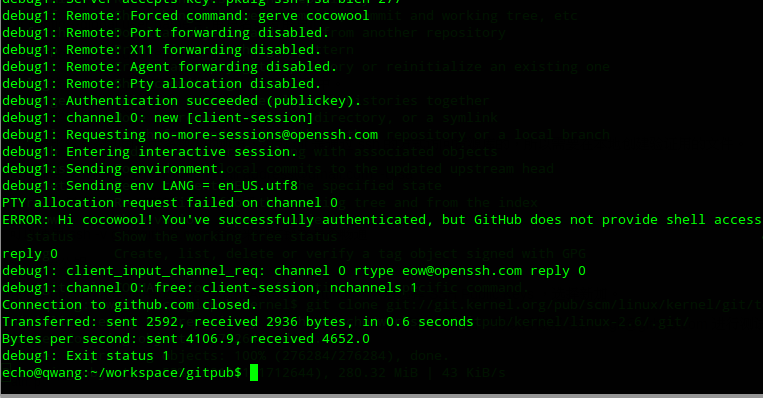
\includegraphics[scale=0.5]{figures/github.png}
\caption{github连接建立成功}\label{github}
\end{figure}

(5)配置显示颜色

\verb"$ git config --global color.status auto"

\verb"$ git config --global color.diff auto"

\verb"$ git config --global color.branch auto"

\verb"$ git config --global color.interactive auto"

(6)中文乱码的解决方法

在bash提示符下输入:

\verb"$ git config --global core.quotepath false"

core.quotepath设为false的话,就不会对0×80以上的字符进行quote。中文显示正常。

然后输入下面命令:

\verb"$ git config --global gui.encoding utf-8"
\verb"$ git config --global i18n.commitencoding utf-8"
\verb"$ git config --global i18n.logoutputencoding gbk"

\subsection{安装perl}
\verb"$ sudo apt-get install perl"

\subsection{安装GEM5}
(1) 将下载的gem5-stable-aaf017eaad7d.tar安装包解压,文件夹重命名为gem5\_stable。

(2) 因为SCons是用Python编写的,所以你必须在使用SCons之前安装好Python (2.7.5)。

(3) 安装scons (2.1以上)

\verb"$ sudo apt-get install scons"

(4) 安装swig (2.07以上)

\verb"$ sudo apt-get install swig"

(5) 安装zlib (1.2.8以上)

\verb"$ sudo apt-get install zlib"

(6) 安装M4

先将下载的m4-1.4.17.tar.gz解压:tar -xzvf m4-1.4.17.tar.gz解压之后的文件夹 m4-1.4.17放到gem5\_stable目录下cd m4-1.4.17
执行命令:

\verb"$ sudo ./configuresudo make install"

(7) 安装protobuf

将下载的安装包解压后进入源代码目录
\begin{verbatim}
  ./configure
  sudo make install
\end{verbatim}

(8) 安装libprotobuf-dev

\verb"$ sudo apt-get install libprotobuf-dev"

(9)	安装libgoogle-perftools-dev

\verb"$ sudo apt-get install libgoogle-perftools-dev"

(10)	编译gem5:cd gem5-stable

\verb"$ sudo mkdir build"

指定编译的选项及目标文件,例如:

scons build/ALPHA/gem5.opt

如果出现如下错误:

错误:can't find Python.h header in ['/usr/include/python2.7']解决:sudo apt-get install python-dev

(11) 测试SE模式下的Hello World

在gem5目录下输入命令
\begin{verbatim}
./build/ALPHA/gem5.opt ./configs/example/se.py -c tests/test-progs/hello/bin/alpha/linux/hello 
gem5 Simulator System.  http://gem5.org
gem5 is copyrighted software; use the --copyright option for details.

gem5 compiled Nov 22 2013 21:02:57
gem5 started Nov 22 2013 21:06:19
gem5 executing on ubuntu
command line: ./build/ALPHA/gem5.opt ./configs/example/se.py -c tests/test-progs/hello/bin/alpha/linux/hello
/home/hu/gem5-stable/configs/common/CacheConfig.py:48: SyntaxWarning: import * only allowed at module level
  def config_cache(options, system):
Global frequency set at 1000000000000 ticks per second
warn: CoherentBus system.membus has no snooping ports attached!
0: system.remote_gdb.listener: listening for remote gdb #0 on port 7000
**** REAL SIMULATION ****
info: Entering event queue @ 0.  Starting simulation...
info: Increasing stack size by one page.
Hello world!
hack: be nice to actually delete the event here
Exiting @ tick 3233000 because target called exit()
\end{verbatim}
安装成功!

(12) 在full system下模式下运行alpha编译的测试程序

在gem5-stable根目录下创建dist目录,并在该目录中创建alpha目录,并将下载的m5-system-2.03.tar.bz2解压,将其中的binaries和disks目录放在dist/alpha目录中。

修改GEM5/config/common/SysPath.py 文件:

把exceptKeyError: path = [ '/dist/m5/system', '/n/poolfs/z/dist/m5/system  

修改成  
  except KeyError: path = [ '/dist/m5/system', ' /home/happy/gem5-stable/dist/alpha' ]

然后编译gem5

~/gem5-stable \$ scons ./build/ALPHA/gem5.opt

可以通过 GEM5/m5out/system.terminal查看启动linux内核的monitor进程。

运行模拟的linux系统

./build/ALPHA/gem5.opt ./configs/example/fs.py  

将看到如下界面
\begin{verbatim}
  gem5 Simulator System. http://gem5.org
  gem5 is copyrighted software; use the --copyright option for details.
  gem5 compiled Jul 13 2013 15:50:46
  gem5 started Jul 13 2013 15:53:18
  gem5 executing on jsi-desktop
  command line: ./build/ALPHA/gem5.opt ./configs/example/fs.py
  Global frequency set at 1000000000000 ticks per second
  info: kernel located at: /home/wyj2/gem5-stable/dist/binaries/vmlinux
  Listening for system connection on port 3456
        0: system.tsunami.io.rtc:Real-time clock set to Thu Jan  100:00:00 2009
  warn: CoherentBus system.membus has no snooping ports attached!
  0: system.remote_gdb.listener: listening for remote gdb #0 on port 7000
  **** REAL SIMULATION ****
  info: Entering event queue @ 0. Starting simulation...
  warn: Prefetch instructions in Alpha do not do anything
  warn: Prefetch instructions in Alpha do not do anything
\end{verbatim}
  
开启另外一个ssh界面,使用M5Term来与simulatedsystem进行交互
\begin{verbatim}
  ~/gem5-stable$cd ./util/term  
  ~/gem5-stable$make  
  ~/gem5-stable$sudo make install  
  ~/gem5-stable$m5term localhost 3456 
\end{verbatim}  

这样就进入了模拟出来的系统:
\begin{verbatim}
  #ls后就看到如下:
  # ls
  benchmarks  etc        linuxrc     modules     sys        var
  bin         iscsi       lost+found  proc       tmp
  dev         lib         mnt         sbin        usr
  5、在模拟系统中运行一个测试程序试试:
  #cd benchmarks
  #ls
  将看到如下几个测试程序:
  aio-bench           netperf-bin         surge
  micros              pthread_mutex_test
  #./pthread_mutex_test2 2
  运行结果如下:
  Using 2 threadsfor 2 iters
  Counter value is 4
  #
\end{verbatim}

现在以将GEM/tests/test-progs/hello/bin/alpha/linux/hello,mount进模拟的系统为例,讲述如何将编译好的程序mount进被模拟的系统。

1、将hello文件拷贝到当前路径/gem5-stable\$ cp./tests/test-progs/hello/bin/alpha/linux/hello ./hello  

2、~/gem5-stable\$ sudo mount -o,loop,offset=32256 ./dist/disks/linux-latest.img /mnt  

关于偏移量32256请参考链接:http://my.oschina.net/toyandong/blog/65002  

3、显示一下/mnt,可以看到挂载好的操作系统  
\begin{verbatim}
~/gem5-stable$ ls/mnt  
benchmarks  dev iscsi  linuxrc     mnt     proc  sys  usr  
bin         etc lib    lost+found  modules sbin  tmp  var  
\end{verbatim}

4、  在使用linux的image文件之前,应该执行umount操作。  

~/gem5-stable\$ sudo umount /mnt  

5、  重新开启模拟的linux,进入模拟的linux (参考本文 “运行” 中的2和3)  
\begin{verbatim}
    #ls  
  可以看到我们添加的testGem5目录
  benchmarks  etc        linuxrc     modules     sys        usr
  bin         iscsi       lost+found  proc       testGem5   var
  dev         lib         mnt         sbin        tmp
\end{verbatim}

6、cd testGem5

\verb"$ sudo ./hello"

执行结果:

\verb"Hello world!"

(13)在full system模式下运行x86程序的方法可以参考下面的网页。

http://blog.csdn.net/wyj7260/article/details/9320113

\subsection{安装Design Compiler}
1.在linux的根目录下建立/usr/synopsys文件夹。

2.在目录下创立以下的目录结构
\begin{verbatim}
  /usr/synopsys 
  |---installer
  |---10.9.3
  |---license
  |---B-2008.09
\end{verbatim}

3.安装installer。将install\_v2.0.rar.Z解压到/usr/synopsys/installer目录即可。

4.解压scl.rar到/usr/synopsys目录中。

5.在终端中以管理员账户下运行下面的命令:
\begin{verbatim}
  	#cd /usr/synopsys/installer/
  	#./installer -gui
\end{verbatim}

便可以调出安装界面,如果运行出错说找不到setup.sh文件,则运行下面的命令安装csh。
\begin{figure}
\centering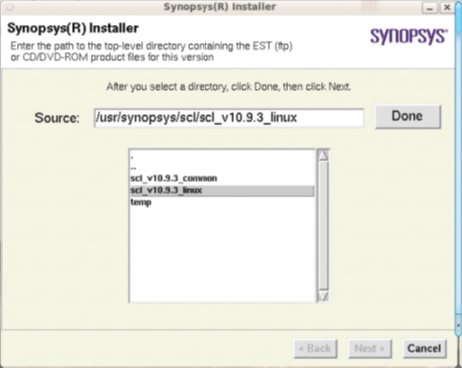
\includegraphics[scale=0.5]{figures/synopsys1.png}
\caption{synopsys安装界面}\label{synopsys1}
\end{figure}
\verb"$ sudo apt-get install csh"

6.选中scl\_v10.9.3\_linux文件后点击下一步,如下图所示:
\begin{figure}
\centering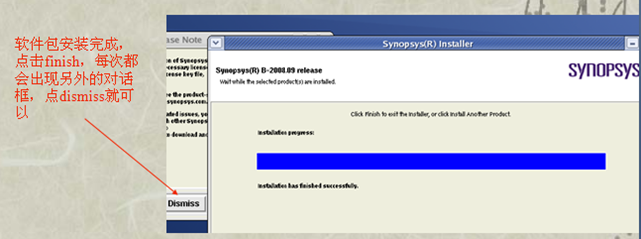
\includegraphics[scale=0.5]{figures/synopsys2.png}
\caption{synopsys安装界面}\label{synopsys2}
\end{figure}
然后一直next,过程中有些选项都不需要管,直到选中安装目标路径/usr/synopsys/10.9.3。软件包每次安装完以后,点击finish以后都会出现一个对话框,不管他直接点击dismiss就可以了。
  
7.以同样的方法把scl\_v10.9.3\_common.tar文件安装到10.9.3目录。在安装过程中可能会出现下面的错误:

cannot find any platform files for product in /usr/synopsys/scl/scl\_v10.9.3\_common platform files.

不用理它,选择No,然后在弹出的对话框中选择next。然后即可完成安装。

8.将Design\_compiler\_2008.09\_linux.rar和Design\_Compiler\_2008.09\_common.rar解压到/usr/synopsys目录下。

9. 以同样的方法将common包和linux包安装好,这两个包的时候最好分开安装,先安装linux包。这两个包都放在/usr/synopsys/B-2008.09下。

10.以同样的方法将vcs-mx\_vD-2009[1].12\_linux.rar和vcs-mx\_vD-2009[1].12\_common.rar解压缩并安装好,这两个包的时候最好分开安装,先安装linux包。这两个包都放在/usr/synopsys/D-2009.12下。

11.在Windows环境下制作DC2008—license和启动配置文件
 
(1)解压dc\_license.rar

(2)进入EFA LicGen 0.4b文件夹,双击里面的licGen.exe,打开packs中的synopsys.lpd文件。
\begin{figure}
\centering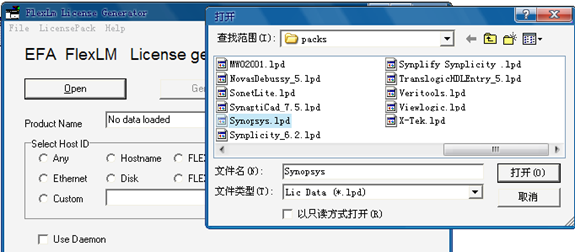
\includegraphics[scale=0.5]{figures/synopsys3.png}
\caption{synopsys安装界面}\label{synopsys3}
\end{figure}

(3)输入mac号,然后点击generate生成synopsys.dat文件。然后点击save将这个文件保存。
\begin{figure}
\centering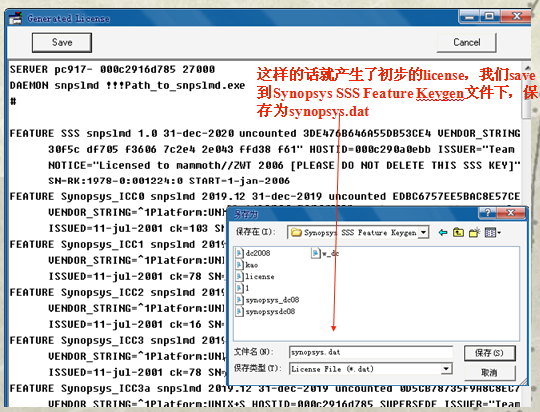
\includegraphics[scale=0.5]{figures/synopsys4.png}
\caption{synopsys安装界面}\label{synopsys4}
\end{figure}

(4)运行sssverify.exe synopsys.dat生成secret code.
  
(5)运行KeyGen.exe,在Secretdata栏中输出上面的secret data码,在host id中填入你的mac地址。然后点击generate命令即可以得到lincense.dat文件。

(6)用记事本打开"synopsys.dat",将第一行修改为:SERVER 主机名 MAC地址27000。其中主机名是Linux系统下的主机名,可在Linux的终端中用"uname -a"命令查看,一般情况下就是@后面的名字;MAC地址就是网卡地址,后面的27000是默认需要的。将"synopsys.dat"第二行改为:

\verb" DAEMON snpslmd /usr/synopsys/10.9.3/linux/bin/snpslmd"

下图就是我得到的license:
\begin{figure}
\centering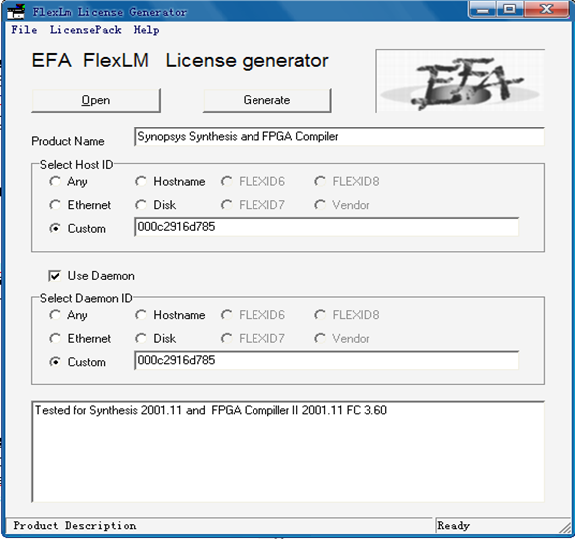
\includegraphics[scale=0.5]{figures/synopsys5.png}
\caption{synopsys安装界面}\label{synopsys5}
\end{figure}

(7)修改FEATURE SSS 部分

打开之前生成的 license.dat(license\\Synopsys SSS Feature Keygen\\license.dat),复制其中的中的 FEATURE SSS 部分,覆盖掉 synopsys.dat 中的 Feature SSS 部分。

(8)至此license 的制作完成,将synopsys.dat拷贝的/usr/synopsys/license 文件夹下。

(9)打开用户目录下的.bashrc 文件,在末尾加上如下内容:
\begin{verbatim}
  export SYNOPSYS=/usr/synopsys
  export SNPSLMD_LICENSE_FILE=27000@happy-ThinkPad_R400
  export LM_LICENSE_FILE=$SYNOPSYS/license/synopsys.dat
  export PATH=$SYNOPSYS/B-2008.09/bin:$SYNOPSYS/D-2009.12/bin:$PATH
  export VCS_HOME=$SYNOPSYS/D-2009.12
  alias lmli2="/usr/synopsys/10.9.3/linux/bin/lmgrd -c /usr/synopsys/license/synopsys.dat -l ~/syn_lic.log"
\end{verbatim}

(10)更新.bashrc文件

\verb"$ sudo source .bashrc"

(11)如果vcs启动过程中出现下面的错误:

\verb" bin sh illegal option"

那么运行下面的命令修改/bin/sh的链接
\begin{verbatim}
  #rm –f /bin/sh
  #ln –s /bin/bash /bin/sh
\end{verbatim}

(15)如果在运行vcs时出现下面的错误:

/usr/synopsys/D-2009.12/bin/vcsMsgReport: line 332: /bin/basename: No such file or directory

将Makefile文件中的-full64选项去掉,同时在.bashrc文件中增加下面的代码

export VCS\_ARCH\_OVERRIDE=linux

即可。

(16)如果在64位系统中编译过程中遇到下面的错误:

/usr/include/features.h:324:26: fatal error: bits/predefs.h: No such file or directory

输入下面的命令解决:

\verb"$ sudo apt-get install gcc-multilib g++-multilib"

(17)在编译过程中出现的链接错误是因为gcc版本太高,可以通过下面的命令:
\begin{verbatim}
  #cd /usr/bin
  #ls –l gcc*
  #mv gcc gcc.bak
  #apt-get install gcc-4.4 g++-4.4
  #ln –s gcc-4.4 gcc
  #ls –l g++*
  #mv g++ g++.bak
  #ln –s g++-4.4 g++
\end{verbatim}

(17)如果在64位系统中编译过程中遇到下面的错误:g++ selected multilib '32' not installed

需要安装gcc、g++的multilib包,直接执行下面的命令,会自动安装g++、gcc的multilib包;
\begin{verbatim}
sudo apt-get install g++-4.4-multilib
\end{verbatim}

\subsection{安装Source Insight}
(1) 安装wine

(2) 安装source insight.exe

\verb"$ sudo wine source insight.exe"

(3) 破解

\subsection{安装Codeblocks}
(1) 安装基本编译环境
\begin{verbatim}
  $sudo apt-get install build-essential
  $sudo apt-get install gdb
\end{verbatim}

(2) 安装codeblock
\begin{verbatim}
  $sudo apt-get install codeblocks
  $sudo apt-get install codeblocks-dbg
  $sudo apt-get install wxformbuilder
\end{verbatim}

(3) 安装wxWidgets
\begin{verbatim}
  $sudo apt-get install libwxbase2.8
  $sudo apt-get install libwxbase2.8-dev
  $sudo apt-get install libwxgtk2.8-0
  $sudo apt-get install libwxgtk2.8-dev
  $sudo apt-get install libwxgtk2.8-dbg
  $sudo apt-get install wx-common
  $sudo apt-get install wx2.8-headers
  $sudo apt-get install wx2.8-i18n
  ($sudo apt-get install wx2.8-examples
  $sudo apt-get install wx2.8-doc
\end{verbatim}

(4) 安装完之后,打开Code::Blocks就能直接使用了。我没有进行编译器路径的设置,只是把编译器选择为GCC而已,使用\#include时要用到的一些头文件还是能找到的。在最后的第一个参考文章中说要进行基本编译运行环境的配置,否则工程编译无法通过。就我门前的学习还用不到工程文件,所以就没有配置。

\subsection{安装gtkwave}
\verb"$ sudo apt-get install gtkwave"

\subsection{安装kscope}
(1) sudo add-apt-repository ppa:fbirlik/kscope

(2) apt-get update

(3) sudo apt-get install kscope-trinity
\begin{verbatim}
  The following package was automatically installed and is no longer required:
    gir1.2-unique-3.0
  Use 'apt-get autoremove' to remove them.
  The following extra packages will be installed:
    cscope kdelibs-data-trinity kdelibs4c2a-trinity libarts1c2a-trinity libartsc0-trinity libtqtinterface xbase-clients
  Suggested packages:
    cscope-el fam perl-suid libarts1-akode-trinity
  The following NEW packages will be installed:
    cscope kdelibs-data-trinity kdelibs4c2a-trinity kscope-trinitylibarts1c2a-trinity libartsc0-trinity libtqtinterface xbase-clients
  0 upgraded, 8 newly installed, 0 to remove and 6 not upgraded.
  Need to get 24.1 MB of archives.
  After this operation, 61.8 MB of additional disk space will be used.
\end{verbatim}

\subsection{安装meld}
\verb"$ sudo apt-get install meld"

\subsection{安装markdown编辑器}
\verb"$ sudo apt-get install retext"

默认的显示比较难看,可以为retex指定一个css主题:在~/.config/ReText project/ReText.conf文件中添加以下两行:
\verb"styleSheet=youxia.css"
\verb"userWebKit=true"

为了开启数学支持,可以添加MathJax插件:在~/.config/markdonw-extensions.txt文件中添加以下两行:
\verb"mathjax"
\verb"attr_list"

\subsection{安装cmake}
\verb"$ sudo apt-get install cmake"

\subsection{安装googletest}
\verb"git clone https://github.com/google/googletest.git"

进入\verb"googletest/googletest/"目录,打开CMakeLists.txt文件,将\verb"option(BUILD_SHARED_LIBS \"Build shared libraries (DLLs).\" OFF)"中的OFF改为ON。

\verb"cmake ."

\verb"make"

\verb"sudo cp -a include/gtest /usr/include"

\verb"sudo cp -a libgtest_main.so libgtest.so /usr/lib/"

使用\verb"sudo ldconfig -v | grep gtest"能看到libgtest的相关信息就成功了。

\subsection{支持exFat文件系统}
\verb"sudo apt install exfat-fuse exfat-utils"

\subsection{安装gitlab}
\verb"sudo apt-get install curl openssh-server ca-certificates postfix"
\verb"sudo apt-get install gitlab-ce"
\verb"sudo gitlab-ctl reconfigure"

安装gitlab-runner来执行CI/CD:
\verb"curl -L https://packages.gitlab.com/install/repositories/runner/gitlab-runner/script.deb.sh | sudo bash"
\verb"sudo apt-get install gitlab-runner"
\verb"sudo gitlab-runner register"
在注册过程中,coordinator URL和gitlab-ci token可以在http://localhost/help/ci/quick\_start/README页面找到。gitlab-ci tags要与.gitlab-ci.yml文件中的tag一致。如果注册成功,在项目首页右侧设置->CI/CD Pipelines->Runners activated for this project项目下就可以看到刚才注册的runner了。

有时runner会连接不上,或者在项目仓库->设置->runner里呈灰色,这有可能是runner机器上没有启动gitlab-runner引起的,可以执行ps -ef | grep gitlab看看是否存在gitlab-runner的进程,如果没有则执行gitlab-runner start 命令启动runner服务。

\subsection{安装jenkins}
官网下载jenkens二进制包安装即可,可以在/etc/default/jenkins中修改jenkins的默认端口HTTP\_PORT以防止端口冲突。然后运行下面的命令启动jenkins:
\verb"sudo /etc/init.d/jenkins restart"

\subsection{安装redmine}
下载bitnami-redmine安装包直接安装即可

\subsection{安装docker}
\verb"sudo apt-get install docker docker.io"
\verb"docker pull daocloud.io/daocloud/tensorflow:latest"
\verb"sudo mkdir -p /data/tensorflow/notebooks"
\verb"docker run -it --rm --name myts -v /data/tensorflow/notebooks:/notebooks -p 8888:8888 daocloud.io/daocloud/tensorflow:latest"

打个补丁
\verb"#!/usr/bin/env bash"
\verb"jupyter notebook --no-browser --NotebookApp.token='token1234' > /notebooks/jupyter-notebook.log"

\subsection{安装ncurse库}
ncurses库是编译llvm必须的库
\verb"sudo apt-get install ncurses-dev"
